% Created 2020-05-06 mié 13:47
% Intended LaTeX compiler: pdflatex
\documentclass[a4paper, 12pt]{article}
\usepackage[utf8]{inputenc}
\usepackage[T1]{fontenc}
\usepackage{graphicx}
\usepackage{grffile}
\usepackage{longtable}
\usepackage{wrapfig}
\usepackage{rotating}
\usepackage[normalem]{ulem}
\usepackage{amsmath}
\usepackage{textcomp}
\usepackage{amssymb}
\usepackage{capt-of}
\usepackage{hyperref}
\usepackage{float, amsfonts, commath, mathtools}
\author{Tabaré Pérez}
\date{\today}
\title{Lecture 13 - 7: The K-Means Algorithm: The Big Picture}
\hypersetup{
 pdfauthor={Tabaré Pérez},
 pdftitle={Lecture 13 - 7: The K-Means Algorithm: The Big Picture},
 pdfkeywords={},
 pdfsubject={},
 pdfcreator={Emacs 26.3 (Org mode 9.3.6)}, 
 pdflang={English}}
\begin{document}

\maketitle
Now, you have the cost.

And the next question is, fine, I'm giving partitioning and I'm giving the
representative: How do I find the best?

Because it's exactly what we have in the supervised case when somebody gave you
an objective, and given this objective, you needed to provide a mechanism to
find the best separators that satisfy this objective. So here it's exactly the
same story.

We have the cost now and we need to find a way to find the best partitioning and
the best representatives. Now, as we know, if we have a number of points, how
many different partitions can we produce, meaning how distinct partitions of
size \(K\) we can produce? So this would be exponential in the number of points,
which means that we cannot just go one partition at a time, check the cost, and
go to the next one.

We cannot do this computation explicitly because the search space of partitions
is so large. Therefore, we need to have an algorithm which would tell us how to
navigate in this space to get to the right partitions. So at this point, we
finished talking about a clustering cost and similarity measure. And the only
remaining point for today is actually how, given this cost, we can find the best
partition.

And I will start introducing you now the K-means algorithm, which achieves
exactly this goal.

So the last part of our lecture for today is \textbf{K-MEANS CLUSTERING ALGORITHM}.

So the way I would like to explain you, before I actually write the formulas, I
would like to show you how this algorithm works, how does it defines the
clusters.

And intuitively speaking, what it will do, it will take a selection of points,
the whole space of points, and then randomly assigned the representatives.

Then every representative will draw to itself the participants which are closest
to it.

Now we will have several clouds, which are associated with this representative.
But when this assignment happen, we may decide to select a new representative.

And after the representatives are reassigned, we can now go and draw a different
partitions. And we will continue this process until convergence.

So let me show you how it works in a specific example.

\begin{figure}[H]
\centering
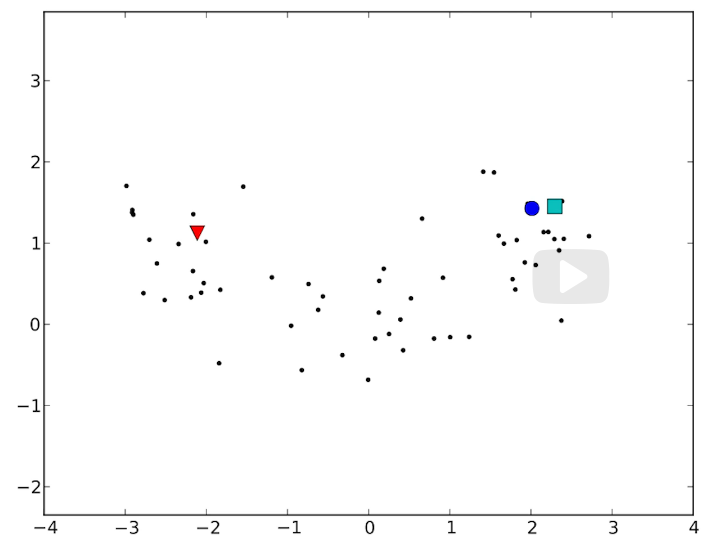
\includegraphics[width=0.5\textwidth]{./pic/k-means-01.png}
\caption{\label{fig:org0c0099c}K-means example}
\end{figure}

So in this particular instance, let's just look at the example before we see the
detail writing of the algorithm.

Let's see how it may be working on a set of points. So let's say here, I am
deciding to identify three clusters. So we would have red, blue, and cyan. This
is our initialization. You can see that these centers were totally randomly
selected.

The next thing that, we will do, we would let every representative to draw the
constituents which are closest to it.

\begin{figure}[H]
\centering
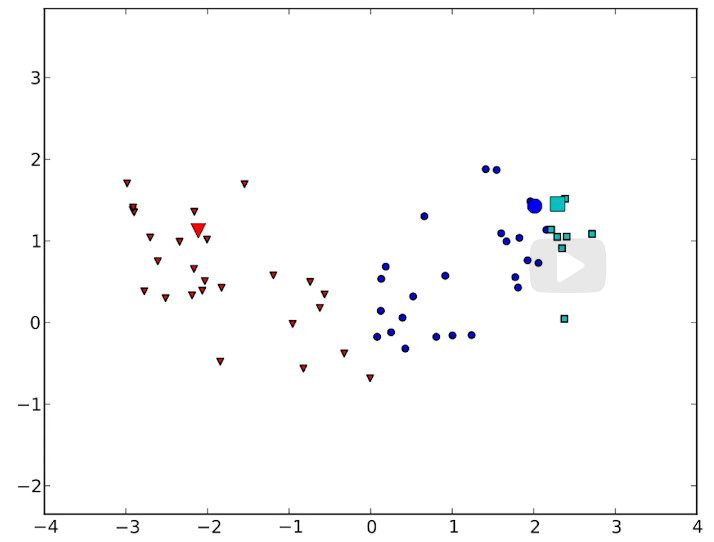
\includegraphics[width=0.5\textwidth]{./pic/k-means-02.png}
\caption{\label{fig:org92ab1a7}K-means example}
\end{figure}

So you see that all the points which are closer to the red representative happen
to be close to. And similarly, you can see the blue and the green ones.

Now even before I will show you the next slide, you can look at it and say, oh,
this is really funny because in this blue cloud the representative, which is
supposed to represent all of them, is somewhere on the outskirts. So the natural
thing is actually to move blue to be really here closer to the center and
similarly to move red to be closer to the center. And that's exactly what we
will do now. And we move them closer.

\begin{figure}[H]
\centering
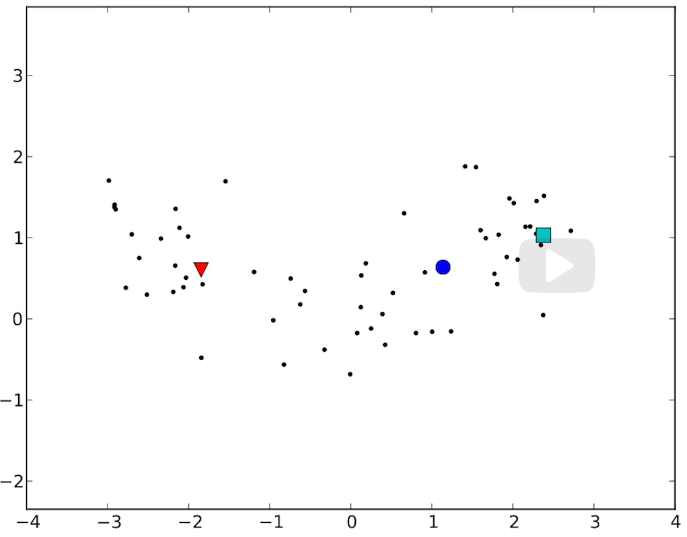
\includegraphics[width=0.5\textwidth]{./pic/k-means-03.png}
\caption{\label{fig:orgf4bdbb3}K-means example}
\end{figure}

So we have a red in the middle, blue in the middle, and cyan closer to its own
original representatives. But now what we can do, we can again find for each
point the representative which is closest to it. And we need to do it anew
because, as you realize here, now since the representative moves, for every
point, they need to decide again who will be the closest representative. And in
this case, we can see, again, there was some movement. We see more red and some
points which were originally maybe blue became red and so on.

\begin{figure}[H]
\centering
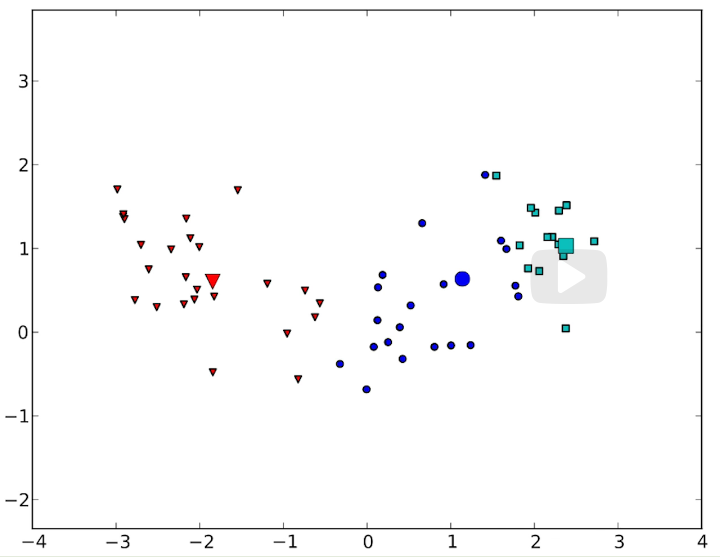
\includegraphics[width=0.5\textwidth]{./pic/k-means-04.png}
\caption{\label{fig:org5e0f8ba}K-means example}
\end{figure}

And we can continue this process again. Blue is located very far from its
constituent. The more natural move is to move in more central location. And
that's exactly what we see here.

\begin{figure}[H]
\centering
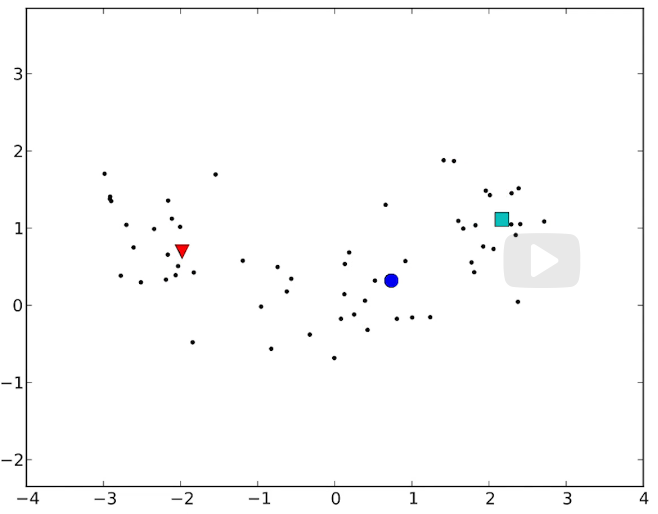
\includegraphics[width=0.5\textwidth]{./pic/k-means-05.png}
\caption{\label{fig:org812d930}K-means example}
\end{figure}

And we can continue this process.

\begin{figure}[H]
\centering
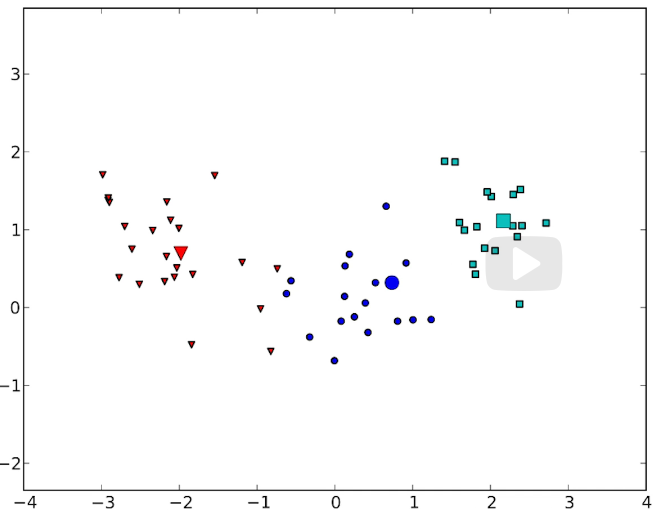
\includegraphics[width=0.5\textwidth]{./pic/k-means-06.png}
\caption{\label{fig:org036a1db}K-means example}
\end{figure}

And eventually, we will generate more stable clustering, which divides all this
points.

\begin{figure}[H]
\centering
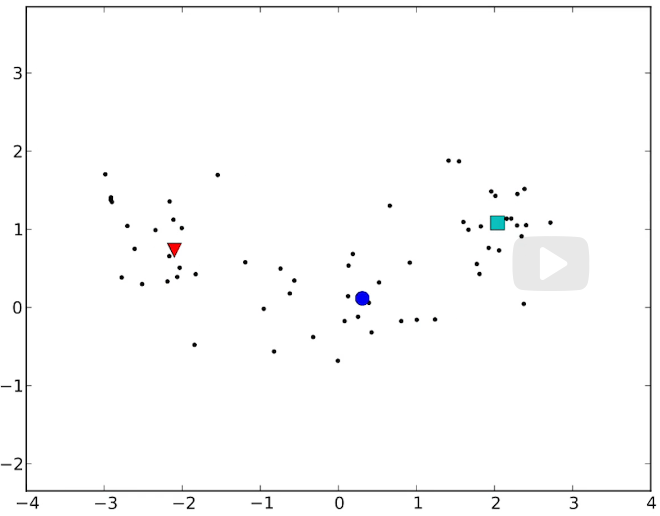
\includegraphics[width=0.5\textwidth]{./pic/k-means-07.png}
\caption{\label{fig:org6a4045d}K-means example}
\end{figure}

So what you've seen here is an example of a run of K-means algorithms.
And we see that there were two parts.

One part is when we randomly assigned the representative, and then every point
was looking for the best one, for the best color for itself.

And then we find we devoted the representative according to that cloud and we
continue this process until convergence.

So now, let's look more formally on how this can be described in terms of our
cost that was just introduced before we went into this example.

So now let's start writing the K-means clustering algorithm. We would follow the
steps that I just demonstrate to you on the example. So K-means clustering we
will start by randomly initializing our representative.

\begin{enumerate}
\item Randomly select \(z^{(1)} \ldots z^{(K)}\). And we will talk shortly about
different strategies of how to do random initialization. But for now, just
you assume it totally randomly selected them.

\item And then we will iterate over the following two steps:

\begin{itemize}
\item 2.1) Given \(z^{(1)} \ldots z^{(K)}\), assigns \(x\)s to the closest \(z\). So
the first step would be, given fixed \(z^{(1)} \ldots z^{(K)}\) the
representatives are given to you, assign \(x_s\) to the closest \(z\). So
at this point, we are given the representatives. We will cycle over all
the our \(x\)s and find the one which is closest. What I would like to do is
actually to write the cost of this assignment:
\end{itemize}
\end{enumerate}

\begin{equation}
\text{cost}(z^{(1)} \ldots z^{(K)})=\sum_{i=1}^{n} \min_{j=1 \ldots K} \norm{x^{(i)} - z^{(j)}}^2
\end{equation}

So our cost would be driven by this \(z^{(1)} \ldots z^{(K)}\) that are fixed,
and what we will have to do, is to go from all the points in our set and then
find for it the closest representative.

So we have the representative from \(1\) to \(K\), \(j\) from \(1\) to \(K\) and now we will
compute \(\norm{x^{(i)} - z^{(j)}}^2\) and so this is our cost.

And we completed this assignment and now we have a new partitions.

Since we have a new partition, we need to reassign that representative which
would be good for that partition:

\begin{itemize}
\item 2.2) Given \(C_1 \ldots C_K\), find the best representatives \(z\).
\end{itemize}

Now what do we mean by the best? We mean the ones which actually minimize our
cost. So in this case, the cost is driven by the partition \(C_1 \ldots C_K\)
and the best we can do here is to find:

\begin{equation}
\text{cost}(C_1, \ldots ,C_K) = \min_{z^{(i)} \ldots z^{(K)}}\sum_{j=1}^{K}\sum_{i \in C_j} \norm{x^{(i)} - z^{(j)}}^2
\end{equation}

over all possible \(z_s\), \(z^{(1)} \ldots z^{(K)}\), those which will minimize
the total cost of the partitioning. So we will go \(j\) from \(1\) to \(K\) and
then for every point in the cluster, we will compute its distance from the
representative.

So again, what are we doing here?

We have the partitions. We will go and try to find the best assignments of the
representatives in such a way that if for every point we compute its distance
from the representative, we achieve the minimum.
\end{document}